% Introduction to additive manufacturing>>>
Additive manufacturing (AM) is described in ISO/ASTM 52900 \cite{international_standard_organization_isoastm_2015} as the "process of joining materials to make parts from 3D model data, usually layer upon layer, as opposed to subtractive manufacturing and formative manufacturing methodologies".
In this first chapter, we will discuss and describe new AM processes or, popularly, 3D printing, which will most likely characterize the manufacturing scenario in upcoming years. Although the adjective "new" may not be quite appropriate, after all. Already from the 1950s - 1960s, before being called AM processes, these processes were called "Rapid Prototyping" (RP). From the name, it is easy to understand why this technology was developed: there was the idea about a lean approach to new product development process, a new approach that would allow to contain costs and reduce time~-~to~-~market. It was only in 1984 and 1986 that the first 3D printing technologies were patented and the possibility of manufacturing a finished object by adding material layer by layer became a reality. The early 2000s were characterized by a push towards the use of these technologies also for large-scale production, trying to unlink RP from the research and development process alone. Indeed, in these years the first cost studies associated with 3D printing usage for mass production were conducted, among which it's worth mentioning \citeauthor{hopkinson_analysis_2003} (\citeyear{hopkinson_analysis_2003}). The real breakthrough for popular 3D printing occurred in the early 2010s, when patents for some polymers used in fused deposition modeling systems (FDM) expired, and there was a real explosion of producers of these polymers and FDM 3D printers. We will discuss about FDM shortly. Nowadays, additive manufacturing is mainly used for the production of small batches of finished products, sometimes even single-unit batches, in the prototyping phase of a new product and in particular contexts which require a very high degree of customization. Moreover, AM processes allow for the creation of complex geometries, objects and patterns that are not achievable with traditional manufacturing processes. As we will see in \textit{Chapter ~\ref{ch:Metal_AM}}, a typical example are lattice structures. 
I want to emphasize from the very beginning that these manufacturing processes do not intend to replace the traditional ones, but rather allow us to expand the limits of what the human being is capable of manufacturing. It's important to understand that additive manufacturing will enable us to obtain components with mechanical functionalities and complexity that were once unimaginable with traditional manufacturing processes, and it could also represent a breakthrough in environmental sustainability by reducing waste of materials.

%%%%%
%%%%%

\section{Additive Manufacturing Process Categories} 
\label{sec:AMproc}
According to ISO/ASTM 52900 \cite{international_standard_organization_isoastm_2015} and \citeauthor{gibson_additive_2015} there are seven different types of AM technologies: vat photo~-~polymerization processes, extrusion-based systems, material jetting, binder jetting, sheet lamination processes, powder bed fusion processes and direct energy deposition processes. Now we will briefly discuss about the different technologies and in \textit{Chapter~ \ref{ch:Metal_AM}} we will focus on AM of metals and powder bed fusion 3d printers.
\begin{itemize}
    \item \textbf{Vat photo-polymerization processes} (VP): VP processes use radiation-curable resins or photopolymers that can be solidified using controlled light sources, usually ultraviolet radiation, but also visible light. Typically, lasers are directed using scanning galvanometers, Digital Micromirror Devices\textsuperscript{TM}, or multiple directional light sources such as the two-photon system or controlled LEDs. The polymers used in this printing technology are usually acrylate~-~based resins or epoxy resins, but also industrial ceramic materials, such as alumina, zirconia and silicone nitride. In recent years, new materials have been developed for the production of investment casting patterns \cite{3d_systems_investment_nodate}, but also high technical performances material such as including cyanate ester, which is used with Carbon Digital Light Synthesis\textsuperscript{TM} to produce finished pieces capable of withstanding high pressures (up to \SIrange[range-phrase = --]{3800}{4000}{\mega\pascal})\cite{carbon_what_nodate}. The major advantages of this technology are the high level of accuracy of the finished products (up to \SI{0.05}{\milli\metre}), relatively high speed of manufacturing, and the variety of print sizes (ranging from very small printers to larger ones, up to \SI{1000}{\milli\metre} x \SI{800}{\milli\metre} x \SI{500}{\milli\metre}). The disadvantages are that the finished prints require significant post-processing, the printers and the process are still quite expensive, material choices are limited to photo-polymers only, and the need to print support structures that are important to prevent the final piece from collapsing.
    \item \textbf{Extrusion-based systems} of \textbf{fused filament fabrication} (FFF): FFF systems selectively extrude material, usually in the form of a filament, through a heated nozzle or orifice. They are also called fused deposition modeling (FDM). The FDM 3D printers we discussed earlier fall into this category and are characterized by a nozzle that is free to move in the horizontal plane and a platform that moves up and down along the z-axis to allow for laerwise material deposition. Typically, materials used with this type of AM are waxes, polyamide, acrylonitrile-butadiene-styrene, polyphenyl sulfone, polycarbonate, ceramics as well as biocompatible or biodegradable materials. The main advantages of FFF systems include their widespread popularity and economic accessibility, as well as the variety of materials that can be used, such as ABS, which provides excellent structural properties, or PLA (polylactic acid), which can be extruded at relatively low temperatures and it is compostable. The drawbacks of this technology include lower print speeds and a lower achievable minimum resolution if compared to other processes, as well as a greater need for post-processing to achieve the desired finishing.
    \item \textbf{Material jetting systems} (MJ): MJ is a technique that allows 3D printing of a piece using tiny droplets of liquid material that are selectively deposited onto a surface. As always, the object is developed adding new material according to a layer-wise logic. In a certain way, material jetting can be seen as the natural evolution of normal 2D inkjet printers but in three dimensions. Just like inkjet printers, in MJ there can be different "cartridges" of materials and colors. In fact, one of the main advantages of MJ is the possibility of printing high-resolution multi-colored or multi-material objects. Initially, the materials used with this technology were waxes, but in recent years the focus has been more on the deposition of acrylate photopolymers, which droplets of materials are solidified with an UV lamp directly attached to print nozzle. The main advantages of MJ are the almost absence of material waste, as the deposition-on-demand process is extremely precise (droplets of \SIrange{25}{120}{\micro\meter} at a rate of 0-2000 drops per second), and the possibility, as mentioned earlier, of using different materials and colors simultaneously. The disadvantages of this solution are mostly the limited number of usable materials, since only polymers and waxes can be used and only materials that are not excessively viscous. Furthermore, the process and equipment required are relatively inexpensive and capable of printing at a sustained speed.
    \item \textbf{Binder jetting systems}: Binder jetting, is very similar to MJ. In binder jetting, a liquid binding agent called "binder" is selectively deposited in small droplets to solidify powdered materials and allow different layers of powder to stick together. Due to the production method, the final objects may not always be suitable for withstanding large structural stresses and often require a long post-processing phase, which could increase variable costs. Binder jetting can be used with both thermo-plastic polymers and metals, as well as ceramic materials. The major advantages of this technology compared to MJ are the ability to use a much wider range of materials and the higher speed of printing. Additionally, it is possible to mix different powders to obtain final objects with different mechanical properties. The disadvantages, as mentioned earlier, are the fact that printed parts may not always be suitable to be used as structural parts and the costly post-processing operations necessary to improve the mechanical characteristics of the finished pieces.
    \item \textbf{Sheet lamination} (LOM): In sheet lamination or laminated object manufacturing (LOM), a 3D printing technique, layers of material are bonded together to form a final object. So, each layer of the final object is made up of a sheet of laminate. There are two different approaches: "bond-then-form" and "form-then-bond". In the first case, the laminate is positioned and bonded to the substrate, and then cut following the model contour. In the second case, the laminate material is first cut and then placed on the substrate and bonded to the underlying layer. LOM techniques allow the usage of wood, thermo-plastic polymers, industrial ceramics, as well as paper, polyvinyl chloride, and composite materials. The major advantages of LOM are the ability to print very large parts quickly and the much lower fixed equipment costs compared to other types of AM processes.
    \item \textbf{Powder bed fusion} (PBF): PBF is also called direc metal laser sintering (DMLS) or selective laser melting (SLM). In these additive manufacturing techniques, a concentrated energy source is used to selectively melt layers of powder. Usually, the energy source is a laser or an electron beam and the materials used can be polyamides, nylons, elastomers, as well as metals such as stainless steel, titanium, aluminum, cobalt, and copper. It's important to note that this AM technique is widely used for direct manufacturing and allows for the production of finished objects with excellent mechanical properties and surface finishes, mostly used in automotive, aerospace, or biomedical industries.
    \item \textbf{Direct energy deposition systems} (DED): in DED, a concentrated heat energy source is used to selectively melt deposited material as soon as it is deposited. Depending on the energy source used, we can further divide the processes into laser metal deposition, electron beam metal deposition, and plasma metal deposition. Moreover, depending on the shape of the material used, we can distinguish between powder-fed and wire-fed systems. Finally, depending on the direction in which the material is fed, we can distinguish between off-axis feeding, in which the material is deposited by a side-mounted incident nozzle, and coaxial feeding systems, in which the powder or wire material is deposited co-axially with the energy beam. The major advantages of DED are that it can be used to add parts to existing components or repair broken components with ease, the ability to print parts with very steep angles without requiring support, the wide range of powders available, the large printing area that can be achieved, and the ability to use various feeders. The disadvantages are that machining and post-processing are often required, overly complex shapes cannot be printed unlike with PBF systems, and overall process accuracy is lower compared to PBF.
    
\end{itemize}
% <<< End of Introduction to Additive Manufacturing

%%%%%
%%%%%


\section{Aim and Structure of the Work}
\label{sec:aimwork}
Additive manufacturing processes for metallic parts, especially the so-called powder bed fusion processes, have been revolutionizing various industries in recent years, including aerospace, automotive, and energy industry. These processes are also used to create components that play a vital role during their use, often critical for safety. Consider, for instance, the importance of the brake system shown in the Fig. \ref{fig:bugatti}. Imagine the repercussions if the braking system failed on a Chiron is speeding at 350 km/h, or if a support, like the one illustrated, may break, causing a \SI{8500}{\metre} fall of a heavy piece. 
\begin{figure}[H]
    \centering
    \subfloat[\label{fig:bugatti}]{
        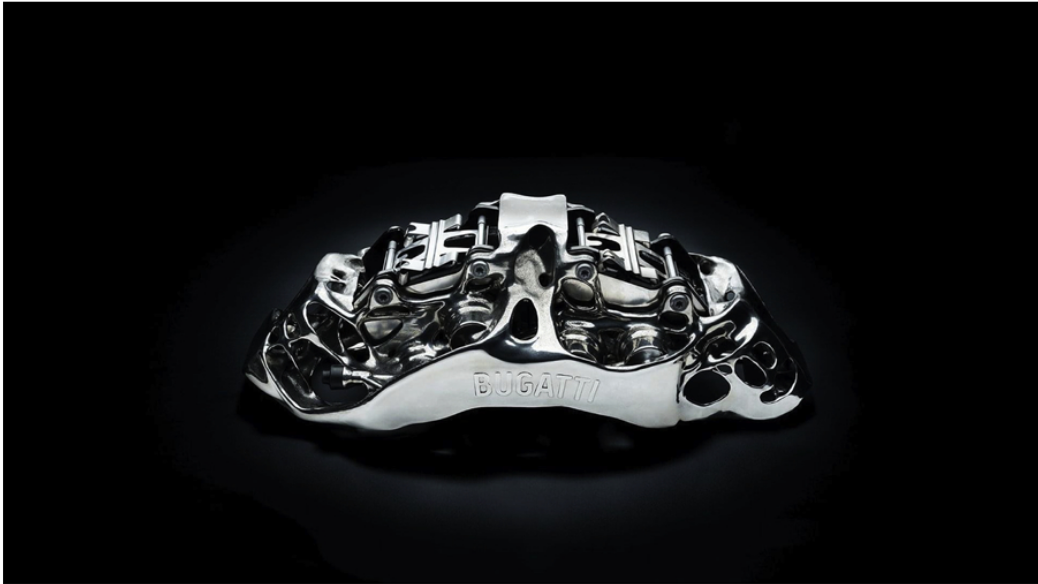
\includegraphics[scale=0.4]{Images/bugatti.png}
    }
    \quad
    \subfloat[\label{fig:supporto}]{
        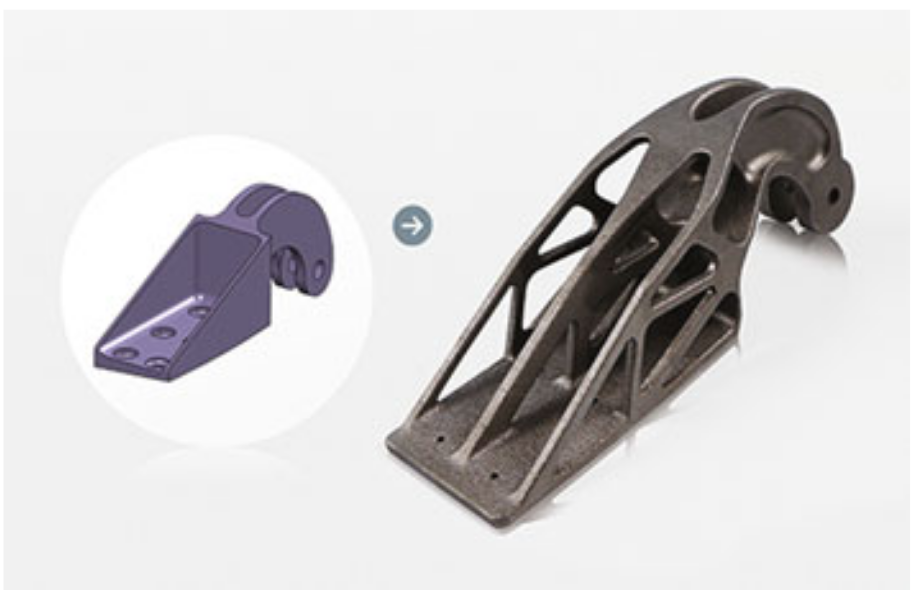
\includegraphics[scale=0.4]{Images/supporto.png}
    }
    \caption[Functional AM part printed in metal.]{On the left, a Bugatti brake caliper, one of the world’s largest functional parts produced in titanium alloy Ti6Al4V by AM. On the right, a support used in aerospace industry. From \citeauthor{du_plessis_beautiful_2019}.}
    \label{fig:funcpart}
\end{figure}
For these reasons, quality control, defect detection, and ensuring the production process adheres to standards are crucial now more than ever. 
Temperature, particularly in additive manufacturing for metallic parts, significantly influences the mechanical properties of the finished product. Indeed, unlike 3D printing using polymers, such as the classic FDM 3D printing, the temperatures reached are much higher, coupled with a much slower cooling process. Anyone who has somehow experienced FDM 3D printing would notice that the filament cools in a matter of seconds. On the other hand, with metallic PBF printing, one must wait considerably longer. Moreover, there are many additional factors that could affect the temperature reached by the material during the PBF printing process and the consequent cooling process.
The aim of this thesis is to present a state-of-the-art review regarding the identification of so-called cold spots and hot spots in PBF processes. These are areas within the print characterized by abnormal temperatures during the printing process, leading to defects in the finished product.
\begin{figure}[H]
    \centering
    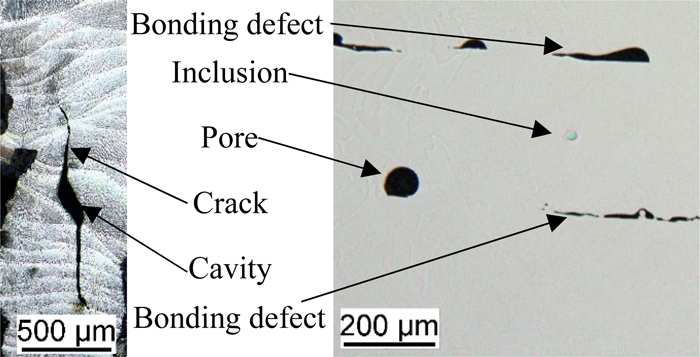
\includegraphics[scale=3.5]{Images/defect.jpeg}
    \caption[Defects in metal AM.]{Defects caused by cold and spots in PBF. From \citeauthor{bernhard_defect_2020}.}
    \label{fig:defect}
\end{figure}

This thesis is structured as follows. In \textit{Chapter~\ref{ch:Metal_AM}}, I will provide a comprehensive description of PBF processes for 3D printing of metal parts, the necessary technologies, materials, and some potential applications. In \textit{Chapter~\ref{ch:hotspot}}, I will outline the most common defects in PBF printing processes for metal parts, with a particular emphasis on the aforementioned cold and hot spots. \textit{Chapter~\ref{ch:state_ot_the_art}} will be a literature review to present the state-of-the-art in defect detection of cold and hot spots. The research methodology is detailed in Appendix~\ref{ap:research}. In \textit{Chapter~\ref{ch:baggingvoronoi}}, I will present an innovative approach that might lead to a deeper understanding of the cold and hot spot phenomenon in the printing processes. \textit{Chapter~\ref{ch:conclusions}} will conclude the thesis and propose some research avenues that, in my opinion, are intriguing. Finally, in Appendix~\ref{ap:Python}, I will present a simple implementation of the algorithm proposed in Chapter~\ref{ch:baggingvoronoi}.